\documentclass[11pt]{article}
\usepackage{natbib,mybigpackage}
\usepackage{algorithm}
%\usepackage{program}
%\usepackage{algpseudocode}
\usepackage{algorithmic}
\usepackage{listings}


\def\xbf{\mathbf{x}}
\def\zbf{\mathbf{z}}
\def\xibf{\mathbf{\xi}}
\title{MA 226 - Assignment Report 5}
\author{Ayush Sharma\\150123046}
\begin{document}
\titlepage
\newpage

\begin{enumerate}
\item[Q 1]   Generate 1000 standard normal variates using standard double-exponential distribution by acceptance-rejection method.
Calculate the necessary constant c, where $\frac{f(x)}{g(x)} \leq c$, $f(x)$ and $g(x)$ are the pdfs of standard normal and standard double-exponential distribution respectively.
Calculate the theoretical and simulated acceptance probability.
How do you justify your generated random numbers are correct ?
Provide as many verification as you can.
\end{enumerate}

\noindent{Solution:}  For generating random number from standard normal distribution by acceptance-rejection method, double-exponential distribution is chosen as our candidate distribution.\\
We can write the probability density function of standard normal distribution as
$$f(x) = f_{Normal}(x) = \frac{1}{\sqrt{2\pi}}e^{-\frac{x^2}{2}}$$
and that of standard double-exponential distribution as
$$g(x) = f_{Double-Exp}(x) = \frac{1}{2}e^{-|x|}$$
Also, we can write the cumulative distribution function of double-exponential distribution as
$$F_{Double-Exp}(x) = \begin{cases} \frac{1}{2}e^x & \text{if $x < 0$} \\ 1 - \frac{1}{2}e^{-x} & \text{if $x \geq 0$} \end{cases}$$
To apply inverse transform method we equate
$$u = F_{Double-Exp}(x) = \begin{cases} \frac{1}{2}e^x & \text{if $x < 0$} \\ 1 - \frac{1}{2}e^{-x} & \text{if $x \geq 0$} \end{cases} \hspace{10mm} \Rightarrow \hspace{10mm} x = \begin{cases} \log(2u) & \text{if $u < \frac{1}{2}$} \\ -\log(2(1 - u)) & \text{if $u \geq \frac{1}{2}$} \end{cases}$$
where $u$ is an observation from Uniform(0,1).\\
We choose c maximizing $\frac{f(x)}{g(x)} = \frac{f_{Normal}(x)}{f_{Double-Exp}(x)} = \sqrt{\frac{2}{\pi}}e^{-\frac{x^2}{2} + |x|}$.\\
Maximum of c will attain at $x = 1$ i.e. $c = \frac{f(1)}{g(1)} = \sqrt{\frac{2e}{\pi}}$.\\
Here,the rejection test $u > \frac{f(x)}{cg(x)}$ can be implemented as $u > \frac{e^{-\frac{x^2}{2}}}{\sqrt{2\pi}}\frac{2}{ce^{-|x|}} = e^{-\frac{1}{2}(|x| - 1)^{2}}$.

\begin{algorithm}[H]
\caption{Generating Random number from standard normal distribution using standard double-exponential distribution by acceptance-rejection method}
\begin{algorithmic}[1]
\STATE Generate $U_1, U_2$ from $\mathcal{U}[0,1]$.
\STATE Generate $Y$ from the following relation $Y = \begin{cases} \log(2U_1) & \text{if $U_1 < \frac{1}{2}$} \\ -\log(2(1 - U_1)) & \text{if $U_1 \geq \frac{1}{2}$} \end{cases}$.
%\STATE  
\IF {$U_{2} \leq \frac{f(Y)}{cg(Y)} = e^{-\frac{1}{2}(|Y| - 1)^{2}}$}
  \STATE  $X = Y$.
\ELSE
  \STATE  return to step 1.
\ENDIF
\end{algorithmic}
\end{algorithm}

\newpage

\noindent{Code for R}

\begin{lstlisting}
f<-function(x) {
  return (exp(-(1 / 2) * ((abs(x) - 1) ^ 2)));
}

genNormal<-function(sample) {
  N<-vector(length = sample);

  set.seed(1);

  j = 0;
  for (i in 1:sample) {
    repeat {
      j = j + 1;
      u<-runif(2, 0, 1);
      if (u[1] < (1/2)) {
        x = log(2 * u[1]);
      }
      else {
        x = -log(2 * (1 - u[1]));
      }
      if (u[2] <= f(x)) {
        N[i] = x;
        break;
      }
    }
  }

  png("1.png");
  hist(N, breaks = 50, col = "light cyan", plot = TRUE);

  return(c(mean(N), var(N), (sample / j)));
}

output<-genNormal(1000);

cat("The sample mean, sample variance, and the simulated acceptance probability are calculated to be", output[1], ",", output[2], ", and", output[3], "respectively.\n");

\end{lstlisting}
\newpage
\noindent{\textbf{Results}:}

The histogram can be shown as :

\begin{figure}[H]
  \centering
  \subfloat[$\xi_{1}$]{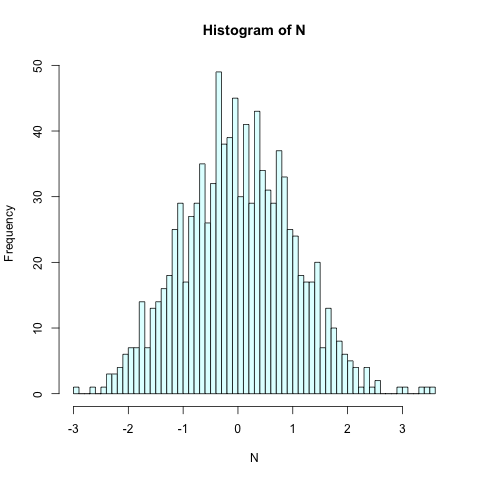
\includegraphics[width=0.7\textwidth]{1.png}}
    \caption{Histogram for n = 1000}
\end{figure}

The sample mean, sample variance, and the simulated acceptance probability are calculated to be 0.01622509 , 1.007402 , and 0.7440476 respectively.
These values are close to the theoretical ones, 0, 1, and $\frac{1}{c} = \sqrt{\frac{\pi}{2e}}$.

\newpage

\begin{enumerate}
\item[Q 2]  Do the same exercise for generating random numbers from half-standard normal distribution using exponential distribution with mean 1 by acceptance-rejection method.
\end{enumerate}

\noindent{Solution:}  For generating random number from half-standard normal distribution by acceptance-rejection method, exponential distribution is chosen as our candidate distribution.\\
We can write the probability density function of standard normal distribution as
$$f(x) = f_{Half-Normal}(x) = \frac{2}{\sqrt{2\pi}}e^{-\frac{x^2}{2}}$$
and that of standard exponential distribution as
$$g(x) = f_{Exp}(x) = e^{-x}$$
Also, we can write the cumulative distribution function of standard exponential distribution as
$$F_{Exp}(x) = 1 - e^{-x}$$
To apply inverse transform method we equate $u = F_{Exp}(x) = 1 - e^{-x}   \Rightarrow   x = -\log(1 - u)$ where $u$ is an observation from Uniform(0,1).\\
We choose c maximizing $\frac{f(x)}{g(x)} = \frac{f_{Half-Normal}(x)}{f_{Exp}(x)} = \frac{\frac{2}{\sqrt{2\pi}}e^{-\frac{x^2}{2}}}{e^{-x}}$.\\
The maximum value will be attained at $x = 1$ which gives $c = \frac{f(1)}{g(1)} = \sqrt{\frac{2e}{\pi}}$.\\
Here,the rejection test $u > \frac{f(x)}{cg(x)}$ can be implemented as $u > e^{-\frac{1}{2}(x - 1)^{2}}$.

\begin{algorithm}[H]
\caption{Generating Random number from half-standard normal distribution using standard exponential distribution by acceptance-rejection method}
\begin{algorithmic}[1]
\STATE Generate $U_1, U_2$ from $\mathcal{U}[0,1]$.
\STATE Generate $Y$ from the following relation $Y = -\log(1 - U_1)$.
%\STATE  
\IF {$U_{2} \leq \frac{f(Y)}{cg(Y)} = e^{-\frac{1}{2}(Y - 1)^{2}}$}
  \STATE  $X = Y$.
\ELSE
  \STATE  return to step 1.
\ENDIF
\end{algorithmic}
\end{algorithm}

\newpage

\noindent{Code for R}

\begin{lstlisting}
f<-function(x) {
  return (exp(-(1 / 2) * ((x - 1) ^ 2)));
}

genHalf_Normal<-function(sample) {
  H_N<-vector(length = sample);

  set.seed(1);

  j = 0;
  for (i in 1:sample) {
    repeat {
      j = j + 1;
      u<-runif(2, 0, 1);
      x = - log(1 - u[1]);
      if (u[2] <= f(x)) {
        H_N[i] = x;
        break;
      }
    }
  }

  png("2.png");
  hist(H_N, breaks = 50, col = "light cyan", plot = TRUE);

  return(c(mean(H_N), var(H_N), (sample / j)));
}

output<-genHalf_Normal(1000);

cat("The sample mean, sample variance, and the simulated acceptance probability are calculated to be", output[1], ",", output[2], ", and", output[3], "respectively.\n");

\end{lstlisting}
\newpage
\noindent{\textbf{Results}:}

The histogram can be shown as :

\begin{figure}[H]
  \centering
  \subfloat[$\xi_{1}$]{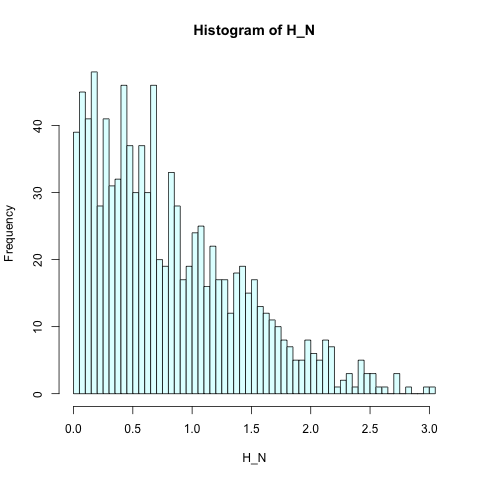
\includegraphics[width=0.7\textwidth]{2.png}}
    \caption{Histogram for n = 1000}
\end{figure}

The sample mean, sample variance, and the simulated acceptance probability are calculated to be 0.8073551 , 0.3755636 , and 0.7541478 respectively.
These values are close to the theoretical ones, $\sqrt{\frac{2}{\pi}}$, $1 - \frac{2}{\pi}$, and $\frac{1}{c} = \sqrt{\frac{\pi}{2e}}$.

\newpage

\begin{enumerate}
\item[Q 3]  Consider the following discrete distribution.
\begin{center}
\begin{tabular}{ cccccc } 
  $j$ & 1 & 2 & 3 & 4 & 5 \\
  \hline
  $p_{j}$ & 0.05 & 0.25 & 0.45 & 0.15 & 0.10 \\
\end{tabular}
\end{center}

a) Generate 10 random numbers from the above probability mass function using usual procedure (inverse transform) of generating random number from discrete distribution defined on finite number of points.
Calculate mean and variance of the generated numbers.

b) Generate 10 random numbers from the same probability mass function by acceptance rejection principle.
Calculate mean and variance of the generated numbers.

\end{enumerate}

\noindent{Solution:}\\
\noindent{a)} For generating random number from given discrete distribution by inverse transform method, we find cumulative distribution function for the given distribution.\\
\begin{center}
\begin{tabular}{ cccccc } 
  $j$ & 1 & 2 & 3 & 4 & 5 \\
  \hline
  $P_f(X = j)$ & 0.05 & 0.25 & 0.45 & 0.15 & 0.10 \\
  \hline
  $P_f(X \leq j)$ & 0.05 & 0.30 & 0.75 & 0.90 & 1.00 \\
\end{tabular}
\end{center}

\begin{algorithm}[H]
\caption{Generating random number from given discrete distribution by inverse transform method}
\begin{algorithmic}[1]
\STATE Generate $U$ from $\mathcal{U}[0,1]$.
%\STATE  
\IF {$U < 0.05$}
  \STATE  $X = 1$.
\ELSIF {$U < 0.30$}
  \STATE  $X = 2$.
\ELSIF {$U < 0.75$}
  \STATE  $X = 3$.
\ELSIF {$U < 0.90$}
  \STATE  $X = 4$.
\ELSE
  \STATE  $X = 5$.
\ENDIF
\end{algorithmic}
\end{algorithm}

\newpage

\noindent{Code for R}

\begin{lstlisting}
P_inv<-function(x) {
  if (x < 0.05) {return(1);}
  else if (x < 0.3) {return(2);}
  else if (x < 0.75) {return(3);}
  else if (x < 0.9) {return(4);}
  else {return(5);}
}

genDiscrete<-function(sample) {
  D<-vector(length = sample);

  set.seed(1);

  for (i in 1:sample) {
    D[i] = P_inv(runif(1, 0, 1));
  }

  png("3_1.png");
  hist(D, breaks = 5, col = "light cyan", plot = TRUE);

  return(c(mean(D), var(D)));
}

output<-genDiscrete(10);

cat("The sample mean, and variance are calculated to be", output[1], ", and", output[2], "respectively.\n");

\end{lstlisting}
\newpage
\noindent{\textbf{Results}:}

The histogram can be shown as :

\begin{figure}[H]
  \centering
  \subfloat[$\xi_{1}$]{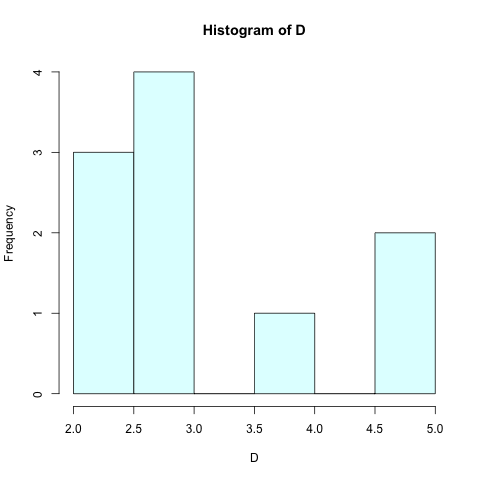
\includegraphics[width=0.7\textwidth]{3_1.png}}
    \caption{Histogram for n = 10}
\end{figure}

The sample mean, and variance are calculated to be 3.2 , and 1.288889 respectively.

\newpage

\noindent{b)} For generating random number from given discrete distribution by acceptance-rejection method, we choose discrete uniform distribution $P_g(X = j) = \frac{1}{5}$, for $j \epsilon \{1, 2, 3, 4, 5\}$.\\
To simulate from this distribution, we generate a uniform random number $u$ and then set $x = j, if \frac{j - 1}{5} \leq u < \frac{j}{5}$.\\
This condition is equivalent to if $(j - 1) \leq 5u < j$, that is $x = \left \lfloor{5u}\right \rfloor + 1$.\\
We choose c maximizing $\frac{P_f(X = j)}{P_g(X = j)} = 5P_f(X = j)$.\\
The maximum value will be attained at $j = 3$ which gives $c = \frac{P_f(X = 3)}{P_g(X = 3)} = 5\times0.45 = 2.25$.\\
Here,the rejection test $u > \frac{P_f(X = j)}{cP_g(X = j)}$ can be implemented as $u > \frac{P_f(X = j)}{0.45}$.


\begin{algorithm}[H]
\caption{Generating random number from given discrete distribution by acceptance-rejection method}
\begin{algorithmic}[1]
\STATE Generate $U_1, U_2$ from $\mathcal{U}[0,1]$.
\STATE Generate $Y$ from the following relation $Y = \left \lfloor{5U_1}\right \rfloor + 1$.
%\STATE  
\IF {$U_{2} \leq \frac{P_f(X = Y)}{cP_g(X = Y)} = \frac{P_f(X = Y)}{0.45}$}
  \STATE  $X = Y$.
\ELSE
  \STATE  return to step 1.
\ENDIF
\end{algorithmic}
\end{algorithm}

\newpage

\noindent{Code for R}

\begin{lstlisting}
p<-function(x) {
  if (x == 1) {return(0.05);}
  else if (x == 2) {return(0.25);}
  else if (x == 3) {return(0.45);}
  else if (x == 4) {return(0.15);}
  else {return(0.1);}
}

genDiscrete<-function(sample) {
  D<-vector(length = sample);

  set.seed(1);

  for (i in 1:sample) {
    repeat {
      u<-runif(2, 0, 1);
      x = (floor(5 * u[1]) + 1);
      if (u[2] <= (p(x)/0.45)) {
        D[i] = x;
        break;
      }
    }
  }

  png("3_2.png");
  hist(D, breaks = 5, col = "light cyan", plot = TRUE);

  return(c(mean(D), var(D)));
}

output<-genDiscrete(10);

cat("The sample mean, and variance are calculated to be", output[1], ", and", output[2], "respectively.\n");

\end{lstlisting}
\newpage
\noindent{\textbf{Results}:}

The histogram can be shown as :

\begin{figure}[H]
  \centering
  \subfloat[$\xi_{1}$]{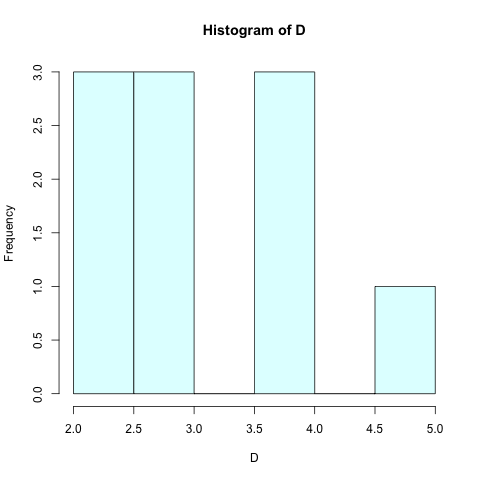
\includegraphics[width=0.7\textwidth]{3_2.png}}
    \caption{Histogram for n = 10}
\end{figure}

The sample mean, and variance are calculated to be 3.2 , and 1.066667 respectively.

\end{document}

%#Made by Ayush Sharma#
%#Signed as AShar#